
\section{Intégration de moteurs dans le SI}

\begin{frame}{Moteurs de recherche}
  Moteurs libres
  \begin{itemize}
    \item Apache Solr (Lucene)
    \item {\color{red}ElasticSearch (Lucene)}
    \item Sphinx
    \item Xapian
  \end{itemize}
  \medskip
  Moteurs commerciaux
  \begin{itemize}
    \item Google Search Appliance
    \item Exalead, Qwant
    \item Amazon CloudSearch
    \item Microsoft Azure Search, Bing
  \end{itemize}
\end{frame} % ending frame Moteurs de recherche

\begin{frame}{Bases documentaires et moteur de recherche}
  \begin{center}
    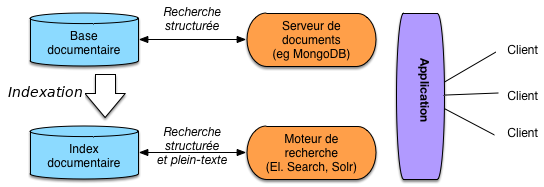
\includegraphics[width=13cm]{../figures/archi-ri2.png}
  \end{center}
\end{frame}

\begin{frame}{Bases documentaires et moteur de recherche}
Un scénario typique :
\begin{itemize}
  \item une recherche par mot-clé dans un site
  \item Les données du site sont gérées classiquement par une base documentaire
    (MySQL, Postgres, MongoDB)
  \item On extrait de la base tous les textes à \alert{indexer} et on en fait
    des documents ES/Solr, à qui on les confie
  \item Ce dernier se charge alors de répondre quand un utilisateur emploie un champ de recherche.
\end{itemize}
\end{frame} % ending frame 


\begin{frame}{Bases documentaires et moteur de recherche}

Un système comme ElasticSearch est consacré à la \alert{recherche},
    c'est-à-dire la lecture la plus efficace possible de documents.

\vfill

Il s'appuie pour cela sur des structures compactes, compressées,
    optimisées (les \alert{index inversés}) 

\vfill

Ce n'est pas (pas forcément) un très bon outil pour les autres fonctionnalités
    d'une base de données :
    \begin{itemize}
      \item Le stockage par exemple n'est ni aussi robuste ni aussi stable.
      \item Mises à jour coûteuses et asynchrones
    \end{itemize}

\end{frame} % ending frame 

\begin{frame}{Présentation d'Elasticsearch}
  Elasticsearch est un moteur de recherche basé sur Lucene
  \begin{itemize}
    \item grande communauté d'utilisateurs
    \item open source, profite de la recherche dans le domaine sur Lucene
    \item utilisé par de grands opérateurs du Web sur des collections immenses
  \end{itemize}
  \medskip
  En fait, plusieurs composants dont :
  \begin{itemize}
    \item Logstash, l'ETL, pour extraire, transformer et charger les données
    \item ElasticSearch, le moteur lui-même
    \item Kibana, pour produire des tableaux de bords de surveillance
  \end{itemize}
\end{frame}

\begin{frame}[fragile]{Installer ElasticSearch 2.4 et le plugin Kopf}

  \begin{minted}[frame=lines,                                                     
               baselinestretch=1.3,                                              
               fontsize=\footnotesize,                                          
               framesep=2mm]{bash}
docker run -d --name es1  -p 9200:9200 -p 9300:9300 elasticsearch:2.4 \
   -Des.index.number_of_shards=1 \
   -Des.index.number_of_replicas=0
\end{minted} 
\bigskip
  \begin{minted}[frame=lines,                                                     
               baselinestretch=1.3,                                             
               fontsize=\footnotesize,                                          
               framesep=2mm]{bash}
   $  docker ps -a
   $  docker docker exec <containerId> plugin install lmenezes/elasticsearch-kopf

   # Adresse IP de votre ElasticSearch
   $ ip="$(docker inspect --format '{{ .NetworkSettings.IPAddress }}' es1)"
   $ echo $IP
\end{minted} 

\end{frame}

\begin{frame}[fragile]{Un premier document}

  Télécharger la liste des films sur \url{http://webscope.bdpedia.fr/index.php?ctrl=xml}
  (Exports, Listes des films complets, un fichier JSON par film ZIPpé)
  \begin{minted}[frame=lines,                                                     
               baselinestretch=1.3,                                              
               fontsize=\footnotesize,                                          
               framesep=2mm]{bash}
$ unzip movies-json.zip
$ cd movies-json/
<EDITER le fichier pour enlever le champ id>
\end{minted} 
\end{frame}
\begin{frame}[fragile]{Notre premier document}
  \begin{minted}[baselinestretch=.9, fontsize=\footnotesize]{json}
{
  "title": "Vertigo",
  "year": 1958,
  "genre": "drama",
  "summary": "Scottie Ferguson, ancien inspecteur de police, est sujet au vertige depuis qu'il a 
              vu mourir son collègue. Elster, son ami, le charge de surveiller sa femme, 
              Madeleine, ayant des tendances suicidaires. Amoureux de la jeune femme Scottie ne 
              remarque pas le piège qui se trame autour de lui et dont il va être la victime... ",
  "country": "DE",
  "director": 	{
    "_id": "artist:3",
    "last_name": "Hitchcock",
    "first_name": "Alfred",
    "birth_date": "1899"	
  },
  "actors": [
  {
    "_id": "artist:15",
    "first_name": "James",
    "last_name": "Stewart",
    "birth_date": "1908",
    "role": "John Ferguson"	
  },
  {
    "_id": "artist:282",
    "first_name": "Arthur",
    "last_name": "Pierre",
    "birth_date": null,
    "role": null	
  }
  ]
}
\end{minted} 
\end{frame}

\begin{frame}[fragile]{Un premier document}
  \begin{minted}[frame=lines,
               baselinestretch=1.3,
               fontsize=\footnotesize,
               framesep=2mm]{bash}
# Utiliser l'API REST pour mettre le document dans ElasticSearch
$ curl -X PUT http://localhost:9200/nfe204/movies/movie:1 --data-binary @movie_1.json

# constater que l'on a bien un index appelé nfe204
$ firefox http://localhost:9200/_plugin/kopf/

# Ensuite, récupérer le document avec curl :
$ curl -X GET http://localhost:9200/nfe204/movies/movie:1
\end{minted}
\end{frame}


\begin{frame}[fragile]{D'autres documents}
  \begin{minted}[frame=lines,                                                     
               baselinestretch=1.3,                                             
               fontsize=\footnotesize,                                          
               framesep=2mm]{bash}
$ wget http://b3d.bdpedia.fr/files/movies-elastic.json

# Utiliser l'API REST et l'interface bulk pour déposer les documents dans ElasticSearch
$ curl -XPUT http://localhost:9200/_bulk --data-binary @movies-elastic.json $
# constater avec Kopf que l'on a 4849 documents importés dans l'index nfe204.
\end{minted} 
\end{frame}


